\documentclass[journal]{IEEEtran}

\usepackage{times}
\usepackage{epsfig}
\usepackage{graphicx}
\usepackage{amsmath}
\usepackage[psamsfonts]{amssymb}
\usepackage{url}
\usepackage[pagebackref=true,breaklinks=true,letterpaper=true,colorlinks,bookmarks=false]{hyperref}

\begin{document}

\title{Surface EMG for Force Control of\\Mechanical Hands}

\author{Claudio~Castellini, Patrick van der Smagt, Giulio~Sandini
\thanks{C. Castellini \emph{(corresponding author)}
  is with the LIRA-Lab, University of Genova,
  viale F. Causa, 13, 16145 Genova, Italy.
  e-mail: claudio.castellini@unige.it.}%
\thanks{P. van der Smagt is with the DLR, German Aerospace Center,
  Institute of Robotics and Mechatronics, Oberpfaffenhofen, Germany.
  e-mail: smagt@dlr.de.}%
\thanks{G. Sandini is with the Italian Institute of Technology,
  via Morego, 30, 16100 Genova, Italy.
  e-mail: giulio.sandini@iit.it.}%
}

\maketitle

\begin{abstract}
  abstract
\cite{v-edbed-82}

\end{abstract}

\begin{IEEEkeywords}
advanced prosthetics, machine learning, EMG, force control, mechanical hands
\end{IEEEkeywords}

\IEEEpeerreviewmaketitle

\section{Introduction}
\label{sec:introduction}
Active prosthetic hands, driven by a motor to open and close the
``claw,'' have been around for many years.  Recently, however,
advances in mechatronics have improved such hands and currently
various prosthetic hands with 3 or more active degrees of freedom are
being put on the market.  Such hand developments are a result of
various robotic hands which are highly humanoid, light and gifted with
a number of degrees of freedom. Attempts in this sense include, e.g.,
the DLR prosthetic hand (\cite{Hua2006}---see Figure
\ref{fig:DLRHandII}), the CyberHand project \cite{cyberhand}, and the
i-LIMB hand by Touch Bionics \cite{ilimb}.

\begin{figure}
  \begin{tabular}{cc}
    \includegraphics[height=0.12\textheight]{figs/DLRHand-Ball-comp.jpg} &
    \includegraphics[height=0.12\textheight]{figs/DLR-Prothese.jpg}
  \end{tabular}
  \caption{(left) The DLR Hand II. (right) The DLR prosthetic hand.}
  \label{fig:DLRHandII}
\end{figure}

Still, a general sense of frustration impends, as far as
\emph{control} of the prosthesis is concerned. As a matter of fact,
given the current state of the art, it is basically impossible for the
patient to precisely command the prosthesis what to do; whereas,
operating a hand requires a fine control down to the level of the
single fingers. First of all, presented with a certain task such as
turning a door handle or grabbing a car key, the patient must be able
to enforce the correct grasping type; this involves the activation of
some joints only, and in particular positions. Secondly, the amount of
force involved in the grasp must be controlled, so that it is possible
to grab, e.g., both a hammer without letting it slip and an egg
without breaking it.

To this end, two types of interfaces between the patient and the
prosthesis have been developed or are being studied: \emph{invasive}
and \emph{non-invasive}. The former gather control signals directly
from the user's nervous system, either via brain implants or surgical
use of electrodes. Quite obviously, invasive interfaces are supposed
to deliver a high signal quality, since the signals can be gathered
exactly in the right spots; but they involve surgery and all related
sterility (and psychological) issues. On the other hand, non-invasive
interfaces are easier to handle, manufacture and implant, but require
a much better signal conditioning, since they usually work with
surface (skin) signals or vision and gaze tracking.

In the context of non-invasive interfaces for controlling mechanical
hands, a concrete possibility arises from \emph{forearm surface
electromyography} (EMG), a technique by which muscle
activation potentials are gathered by electrodes placed on the
patient's forearm skin; these potentials can be used to track which
muscles the patient is willing to activate, and with what force.
Surface EMG is therefore, in principle, a cheap and easy way of
detecting what the patient wants the prosthesis to do.

Still, the EMG signal suffers from a number of problems, among which
the unprecise placement of the electrodes, signal drifting and change
due to sweat formation and muscular fatigue and cross-talking among
deep and superficial muscles. It seems, though, that good results can
be obtained via \emph{machine learning} techniques, as shown in, e.g.,
\cite{smagt}. In machine learning, one tries to approximate an unknown
function given its values in a number of samples; the application to
the current problem is exactly that of building a map relating EMG
activation potentials and muscle force, and therefore hand finger
movements.

Such a system must be highly adaptive, accurate and fast---possibly,
able to run in real time, as the patient is wearing the prosthesis.
Another very desirable characteristic is that the system should learn
automatically as the patient moves, being able to understand when new
portions of the input space are being explored, i.e., what new
movements are required of the prosthesis. But so far machine learning
applied to surface EMG has only been able to classify hand postures.
For example, the surface EMG signal can be used to detect whether the
patient is attempting a cylindric grasp or a two-finger grip
\cite{ekvall}; but no indication about the amount of force involved in
the grasping act is detected.

In this paper we show a rather detailed analysis of what machine
learning can do when applied to such a problem. Over several days, we have
gathered forearm surface EMG data while an able-bodied human subject
was gripping in four distinct ways a force sensor; we have then
trained three different machine learning systems to guess, from the
EMG signal,
\begin{enumerate}

  \item what kind of grasp the subject was doing, e.g., thumb and
    index finger, thumb and middle finger, thumb and ring finger or
    thumb and all other fingers; and

  \item how much force the subject was exerting, in order to
    understand whether the grasp was, e.g., a power grasp or rather a
    precision grip. Surprisingly, as far as we know, nobody has ever
    attempted so far to solve this problem, although it is well-known
    that the EMG is related to the force a muscle is exerting.

\end{enumerate}

The three approaches we have experimented with are:
(a) a simple feed-forward neural network with one hidden layer,
(b) a Support Vector Machine with radial basis function kernel
\cite{BGV92}, and (c) Locally Weighted Projection Regression
\cite{lwpr}. Our analysis consists of a preliminary phase in which
several models have been built in a batch fashion, in order to
understand how to deal with the non-stationarity of EMG. The most
interesting challenge has been how to filter out unwanted data, at the
same time keeping a high overall accuracy, both in classification and
regression. Later on, based upon the results obtained in the
preliminary phase, we have developed a simple but effective procedure
for selecting a subset of the samples on-the-fly, called \emph{Online
Uniformisation} (OU).

OU is based upon the simple idea of keeping a minimum inter-sample
Euclidean distance, in order to uniformly sample the input space. The
selected samples are then used to periodically re-train the system,
and check that it has adapted to the new data. The training sets thus
obtained are remarkably small and thus usable on-line, and they offer
an excellent trade-off between size and accuracy. In particular, as a
certain parameter is increased, the size of the uniform training sets
decreases polynomially, while the error rate increases only
linearly; therefore one can obtain much smaller training sets (which
means faster or more adaptive machines) by accepting an error rate
which is only linearly worse.

This behaviour appears in both problems highlighted above (the former
involving classification, the latter regression), and for all the
approaches tested. Our numerical results indicate that, in such a
scenario, the type of grasp can be reconstructed with an average
accuracy of $89.67\% \pm 1.53\%$, and the applied force can be
predicted with an average percentage error of $7.89\% \pm 0.09\%$,
meaning $4.5$N over a range of about $57$N.

The paper is structured as follows: after a brief review of relevant
literature, we describe in detail the experiment and the methods used
to tackle it (Section \ref{sec:m&ms}); then we show and comment on the
experimental results, both the preliminary phase and the online
experiments (Section \ref{sec:exp}); lastly, discussion and
conclusions are presented.


\subsection{Related Work}
\label{subsec:relatedwork}
related work.

do we really want to have this section? if so:

\textbf{[[1.Patrick will you help here. do we want to have something
about the forthcoming DLR hand, and how one can in principle control
it using a force signal such as the one we can predict from the EMG?]]}

\textbf{[[2.Patrick again: what approaches have been used in
literature to interface EMG and prosthetic hands, NOT LIMITED to
machine learning?]]}



\textbf{[[Patrick?]}

\section{Materials and Methods}
\label{sec:m&ms}

In this Section we describe in detail the experiment we have
conducted, and the methods we have employed to gather the data, filter
and analyse them.

\subsection{Experimental Setup and Design}
\label{subsec:setup}
The aim of the experiment was to gather forearm surface EMG data in
real-time, and to relate it to $(a)$ the type of grasp applied by the
subject, $(b)$ the force applied by the subject while grasping.

\subsubsection{General setup description}

The experiment consisted of freely, repeatedly pressing a SpaceControl
OFTS force/torque sensor \cite{...} along the large face. Four
different ways of pressing were allowed: opposing the thumb and index,
the thumb and middle, the thumb and ring or the thumb and all other
fingers, at different speeds and with varying force. Four force-sensor
resistors were applied on the subject's hand fingertips (thumb, index,
middle and ring), in order to be able to detect which grasp type was
used at each instant of time. At the same time, $10$ forearm surface
EMG electrodes were applied to the subject's forearm, in order to
gather information about the muscle activation. Figure \ref{fig:setup}
shows some parts of the setup.

\begin{figure*}[!ht] \centering
  \begin{tabular}{ccc}
    \includegraphics[height=0.16\textheight]{figs/OFTS} &
    \includegraphics[height=0.16\textheight]{figs/ottobock} &
    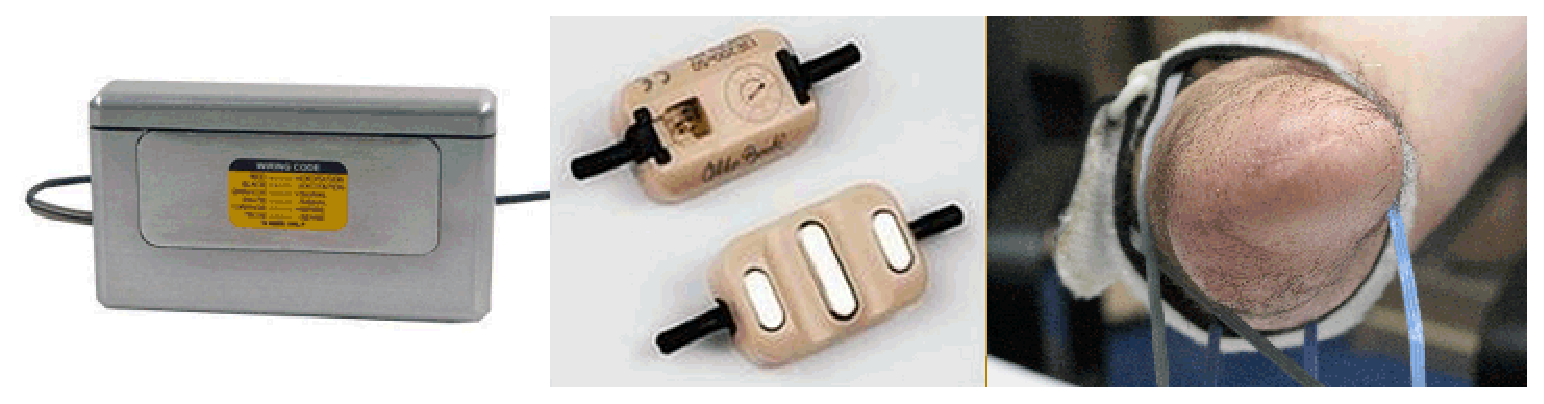
\includegraphics[height=0.16\textheight]{figs/setup} \\
    $(a)$ & $(b)$ & $(c)$ \\
  \end{tabular}
  \caption{The experimental setup. $(a)$ The SpaceControl OFTS
    force/torque sensor, large face up. $(b)$ An Otto Bock 13E200=50
    surface EMG electrode, with the amplification gauge (upper part of
    the Figure) and the three metallic contacts (lower part). $(c)$
    The arm of the subject with the EMG electrodes fitted and held in
    place by elastic bands. Electrodes cables are wired in a box and
    then directed to a National Instruments PCI-6023E analogic/digital
    conversion card (not shown).}
  \label{fig:setup}
\end{figure*}

Numerical data from the EMG and fingertip sensors were gathered at a
sampling rate of $256$Hz using a National Instruments DAQ PCI-6023E
analogic/digital conversion card \cite{...}, mounted on a fast PC
equipped with Windows XP. Data coming from the OFTS sensors was
gathered via the serial port. We ensured that the sampling rate was
high enough and that the card and serial port would respond properly
when requested for data. The data were subsequently synchronised and
saved onto files.

\subsubsection{EMG signal and electrode placement}

The $10$ EMG electrodes were applied to the subject's right forearm,
held in place by elastic bands. The electrodes were
double-differential Otto Bock 13E200=50 models \cite{...}, each one
gifted with an amplification gauge ranging from $2000$ to $100000$
times. Initial qualitative experiments revealed that a safe setting
for the amplification gauge was in the middle of the range,
corresponding to about $14000$ times. This is in agreement with the
EMG signal amplitude predicted in the related literature (see, e.g.,
\cite{deluca}), that is about $100 \mu V$ on average: the voltages our
DAQ card read ranged from slightly more than $0V$ to $3V$.

Six of the electrodes were placed in pairs along the lower face
of the forearm, whereas four of them were applied in pairs on the
upper face. The initial positioning of the electrodes was chosen
following an anatomical guideline \cite{...} in order for them to lie
approximately on top of the muscles which elicit finger movements. As
well, we were inspired by the placement description in \cite{smagt},
which proved to be optimal for Support Vector Machine classification
of hand postures.

As far as the EMG signal is concerned, it must be remarked that it is
subject to remarkable changes depending on, at least, four orders of
factors:

\begin{enumerate}

  \item \emph{the subject.} All forearms are different from one
    another in shape, size and power.

  \item \emph{arm posture.} Besides finger movements and grasping, the
    forearm muscles are also involved in the motion of the arm. The
    EMG signal is therefore likely to change if the forearm is moved
    during signal acquisition, for example when switching from
    pronation to supination.

  \item \emph{electrode placement.} The intensity and quality of the
    EMG signal depends upon a correct placement of the electrode over
    a muscle. In principle, each electrode should be placed over a
    single muscle, precisely on top of the muscle belly, halfway the
    length of the muscle, and always exactly in the same place.

  \item \emph{muscle fatigue.} As the muscles are used more and more,
    continually, fatigue changes the RMS of the EMG signal, calling
    for continual adaptation, at least over a reasonable set of
    different fatigue conditions.

\end{enumerate}

As far as the first problem is concerned, since in a real setting one
person only is expected to train and wear the prosthesis, we have not
investigated multi-subject feasibility of the approach, concentrating
on one subject only, male, aged $35$ and fully able-bodied. Of course,
further investigation is required to check whether the approach can be
transferred to real amputees, by exploiting the residual potential
muscular activation left in their forearm stump. Moreover, independent
multi-subject analysis will have to be carried on, in order to check
that the described approach works with the same accuracy results for
any human being.

In order to overcome the second problem, we instructed the subject to
keep the arm still and relaxed on a table in a confortable position,
with the palm orthogonal to the plane of the table.

Lastly, as far as muscle fatigue and electrode displacement are
concerned: in general, electrodes \emph{cannot} be expected to exactly
lie in the very same position every time the prosthesis is used;
moreover, in a preliminary round of experiments, muscle fatigue was
clearly perceived by the subject during the experiment. In this
framework, the only possibility to overcome these problems is to
explicitly take them into account, gathering enough data to be able to
train the machine under different conditions of electrode displacement
and muscular fatigue.

We then organised the experiment as follows: the subject was
instructed to continually grasp the sensor over a period of time of
three to four minutes; then he was allowed to rest for about two
minutes. This was called a \emph{session}. It was expected that muscle
fatigue would appear already during one session.

Three sessions were gathered without taking the elastic bands off the
subject's forearm, in order \emph{not} to have electrode displacement
within a set of three sessions, that we called a \emph{group}. After
each group, the electrodes and bands were removed and the subject was
allowed for a much longer period of rest, ranging from half an hour to
one hour. During resting in-between groups, the subject could get back
to his normal muscular activity.

Five groups were then gathered during one day; and this procedure was
entirely repeated during another day. This procedure would allow us to
examine a relevant amount of data, gathered along a relatively long
period of time and inder different conditions of muscle fatigue
(within one session) and electrode displacement (between groups).

As an example, Figure \ref{fig:drift} shows the output of electrode
$8$ during three different sessions: $1$ and $2$, belonging to the
same group, and $7$ (moving average over about $10$ seconds). One can
notice strong low-frequency components, essentially drifts due to
muscle fatigue.

\begin{figure*}[!ht] \centering
  \begin{tabular}{ccc}
    \includegraphics[width=0.32\textwidth]{figs/el8_movingAvg_s1} &
    \includegraphics[width=0.32\textwidth]{figs/el8_movingAvg_s2} &
    \includegraphics[width=0.32\textwidth]{figs/el8_movingAvg_s7} \\
    session $1$ & session $2$ & session $7$ \\
  \end{tabular}
  \caption{Typical behaviour of an electrode signal over different
  sessions (moving average over about $10$ seconds. Drifting can be
  clearly seen in the signal, due to muscle fatigue.}
  \label{fig:drift}
\end{figure*}

\subsubsection{Force applied during the grasp}

The OFTS force/torque sensor would output a (negative) numerical value
ranging from $0$ to about $5000$, expressed in fiftieths of a
Newton. After normalisation, the range would be between $0N$ and
$50N$.

\subsubsection{Type of grasp}

The values output by the $4$ force resistor sensors applied onto the
subject's fingertips were monitored in order to understand which kind
of grasp the subject was applying to the sensor. A threshold was
experimentally decided, above which the finger would be in contact
with the sensor. Using this technique, for each instant in time one of
five possible categories was established: $0$, no action; $1$,
grasp by opposing the thumb and index finger; $2$, opposing thumb and
middle; $3$ thumb and ring; and lastly, $4$ grasp by opposing the
thumb and all other fingers.

It must be remarked here that the EMG signal would be altered
immediately at the onset of finger movement, which our setup was
unable to detect. This would result in potential noise in the
categorisation of category $0$.

Figure \ref{fig:targets} shows typical values of the OFTS sensor and
the related categories. One can clearly see that the applied force is
in general higher when grasp type $4$, all fingers involved, is used,
as expected.

\begin{figure*}[!ht] \centering
  \begin{tabular}{cc}
    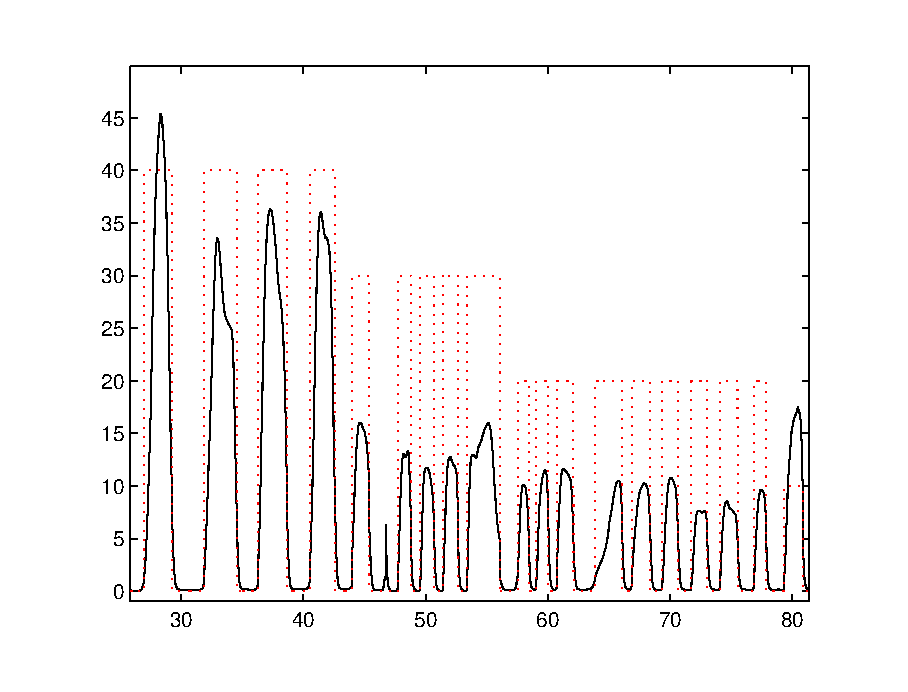
\includegraphics[width=0.45\textwidth]{figs/targets_zoom1} &
    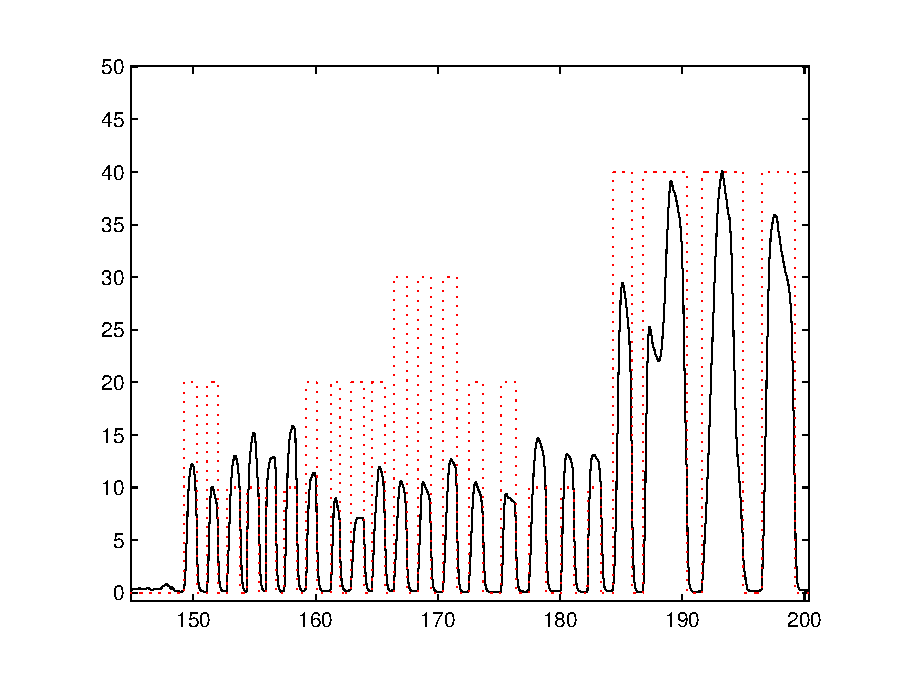
\includegraphics[width=0.45\textwidth]{figs/targets_zoom2} \\
  \end{tabular}
  \caption{Typical values output by the OFTS sensor (black line), and the
    categories evaluated from the fingertip sensors values (red
    line). The Figures are zooms of the same session.}
  \label{fig:targets}
\end{figure*}


\subsection{Data Analysis}
\label{subsec:analysis}
The gathered data was analysed both for classification and
regression. \emph{Classification} is the process by which one wants to
assign a label to each sample in the input space, whereas in
\emph{regression} the target is a real-valued function of the values
of the input samples. Throughout this Section, we will assume that a
set of $l$ points in the input space is available, for which the
target (label or force value) is known; this set will be denoted by
$\{\xx_i,y_i\}_{i=1}^l$ and called \emph{training set}. As well, for
each experiment, a separate set of points, for which the targets are
not known, is assumed to be available, and this will be called the
\emph{testing set}. In general, the performance of a machine is tested
by training it on a training set and then testing it on a testing set,
possibly employing standard measures of the generalisation error, such
as cross-validation.

Taking into account the considerations of the previous Section, we set
the input space to be $\RR^{10}$, that is, one coordinate for each EMG
electrode; therefore, $\xx_i \in \RR^{10}, i=1,\ldots,l$. In the case
of classification, each category representing a grasping type would be
represented as an integer value, that is, $y_i \in \{0,\ldots,4\}
\subset \NN, i=1,\ldots,l$. In the case of regression, the force value
would be directly encoded as a real number, that is, $y_i \in \RR,
i=1,\ldots,l$. Before any analysis, all samples were normalised, as is
customary, by subtracting the mean values and dividing by the standard
deviation, for each input space dimension. No filtering whatsoever was
applied to the input signals, in order to have a more realistic,
delay-free result.

\subsubsection{Neural Networks}

Artificial Neural Networks (NNs or ANNs for short; see, e.g.,
\cite{bishop} for a comprehensive introduction) are probably the most
popular machine learning algorithm nowadays available for both
classification and regression. An ANN is a directed graph in which,
for every node, the weighted sum of the input values is evaluated;
this sum is then used as the argument of an \emph{activation function}
to determine the output of the node. The nodes fed the input values to
the network are called \emph{input layer}, and the nodes whose output
is taken as the output of the network are called \emph{output
layer}. Besides this, in general, an ANN can further have an arbitrary
number of nodes organised in \emph{hidden layers}, gifted with an
arbitrary edge topology.

An ANN is initialised with random weights; then, for every sample in
the training set, the network output is evaluated and its error with
respect to the target is considered. In order to reduce the error
then, a minimisation algorithm is then employed to change the weights
of the network, until the desired precision is reached. If the
generalisation error has been kept small, the network will then be
able to \emph{predict} the targets of the testing samples with a
reasonable accuracy.

For our experiment we strived to keep the ANN as simple as possible.
We then chose a basic feed-forward NN with $10$ units for the input
layer; one hidden layer with $10$ units with sigmoidal arcotangent
activation function; $5$ units in the output layer for classification,
each unit representing one category, and one unit in the output layer
for regression, the unit representing the target force value. The
network was trained via the \textbf{BOH} algorithm and learning
function \textbf{BOHBOH}; the mean-square error (MSE) was used as a
measure of performance. The training phase was stopped arbitrarily
after $30$ epochs. For each experiment, we repeated the training phase
$10$ times, in order to overcome the well-known problem of local
minima, and then gathered the best model found. No measure of
generalisation error was taken into account.

The network was implemented in Matlab, Windows version $7.1.0.246$
(R14) Service Pack 3, running on a bi-processor $1.8$GHz machine with
1GB on-board memory; we used the Matlab Neural Network Toolbox,
version $5.0.1$ (R2006b).

\subsubsection{Support Vector Machines}

Support Vector Machines (SVMs; see, e.g.,
\cite{BGV92,Burges98,Cristianini00}) are a machine learning method
able to determine the best candidate function for a classification or
regression problem, drawn from a functional space induced by the
choice of a binary function between points in the sample space,
$K(\xx_1,\xx_2)$, with $\xx_1, \xx_2 \in \RR^{10}$ in this case. $K$
is called \emph{kernel}. In the most general setting, the function
found is

\begin{equation} \label{eqn:sol}
  f(\xx) = \sum_{i=1}^l \alpha_i y_i K(\xx,\xx_i) + b
\end{equation}

\noindent where $b \in \RR$, whereas the $\alpha_i \in \RR$s are
Lagrangian coefficients obtained by solving a minimisation problem
whose cost functional is guaranteed to be convex. Because of this,
SVMs do not suffer from the problem of local minima; but their
training time is cubic in the number of samples in the training set,
as opposed to ANNs, for which it is \textbf{BOHBOH}.

In order to overcome this problem, which would have made our
experiment unfeasible, we have decided to use a \emph{uniformisation}
strategy on the training sets, before training the machines. The idea
is that, in a real-life set-up such as ours, there can be many input
samples located in the very same region of the input space, with very
similar target values. One obvious case is that of label $0$,
indicating no ongoing grasping: it is intuitively expected that a
large number of samples will be taken in that region of the input
space, since the subject will be in the $0$ condition for a longer
time than all other labels.

Since all functions involved in the experiment are due to human
motion, we can assume that they are continuous and, probably,
derivable up to any arbitrary order. Therefore it makes no sense for
an approach such as SVMs to sample the input space in a non-uniform
way such as that described above. The uniformisation procedure
consists of removing, from a training set, those samples which are too
close to each other, according to a suitable notion of inter-sample
distance.

In order to take into account the different variances of the EMG
electrode values, we have decided to adopt Mahalanobis's distance as
the inter-sample distance \cite{...}. Let $\xx_1, \xx_2 \in \RR^{10}$;
then the Mahalanobis distance between $\xx_1$ and $\xx_2$ is defined
as follows:

$$ MD(\xx_1,\xx_2) = \sqrt{(\xx_1-\xx_2)^T \Sigma^{-1} (\xx_1-\xx_2)} $$

\noindent where $\Sigma$ is the $10$x$10$ covariance matrix, evaluated
on the training set. $MD(\xx_1,\xx_2)$ is a distance in which each
summand is weighted inversely with respect to the variance of the
samples along that dimension of the input space: it is therefore a
measure of distance independent of the variance of the single
electrodes. Notice that if $\Sigma$ is replaced by the identity
matrix, $MD(\xx_1,\xx_2)$ is reduced to the usual notion of Euclidean
distance.

Since checking the inter-sample distance obviously takes a quadratic
time with respect to the number of samples, which was unfeasible, we
adopted an approximated method which was able to remove most, but not
all, samples with an insufficient Mahalanobis distance from any other
sample. After a few initial experiments we set the threshold distance
at $1$. All our experiments with SVMs were then performed on
uniformised training sets, using $5$-fold cross-validation and grid
search to find the optimal values of the standard Gaussian kernel
hyperparameters, $C$ and $\sigma$.

On the other hand, notice that no \emph{testing} set was uniformised,
since it would probably be unfeasible to apply the same procedure in
an on-line setting. Notice, further, that applying uniformisation
resulted in training sets which were considerably smaller than the
original ones, up to about $100$ times smaller.

Lastly, we employed a well-known freely available SVM package,
\emph{libsvm} v2.83 \cite{...}, in the Matlab wrapped flavour.

\subsubsection{Locally Weighted Projection Regression}

\textbf{LWPR - prendi qualcosa dalla rete. spiega gs e cv.}



\section{Experimental Evaluation}
\label{sec:exp}
We conducted two different experiments, one to predict the force measured
by the force sensor and another one to classify the grasp type.
The EMG data were the preprocessed as described in Section \ref{sec:preproc}.

As already mentioned in Section \ref{sec:adapt}, our working assumption is to have
 $N$ pre-trained models stored in memory.
Then new data comes from subject $N+1$ and the system starts
training, to build the $N+1$ model.
The performace is evaluated using unseen data from the subject
$N+1$.
To simulate this scenario and to have reliable estimation of the
performance, we used a leave-one-out approach: 
of the 10 subjects for which we have the data recordings, we train off-line
9 models. These will correspond to the $N$ stored models in memory. The data from the 10th 
remaining subject will be used for the adaptive learning of the $N+1$ model.
The training sequences are random subsets from the entire dataset, that is taken without
considering the order in which they were acquired.
This procedure is repeated 10 times, using in turns all the recorded subjects
for the adaptive learning of the model.

To assess the performance of the proposed adaptation method we compared it
to two baseline methods. The first one, that we call \emph{Prior}, consists in
using only the pre-trained models without updating them with the new training data.
Then we consider only the best performance of the 9 pre-trained models, to consider
the best-case scenario.
The second one, \emph{NoAdapt}, consists in using LS-SVM using only the new data
for training, as it would be in the standard scenario without adaption.
For classification we used the classification rate as a measure of
performance; for regression, the performance index is the correlation coefficient
evaluated between the predicted force signal and the real one. The
choice of the correlation coefficient, as opposed to the more standard
Mean-Square Error, is suggested by a practical consideration: when
driving a prosthesis, or even a non-prosthetic mechanical hand, we are
not interested in the absolute force values desired by the
user/subject, since mechanical hands usually cannot apply as much
force as human hands do, for obvious safety reasons\footnote{or, e.g.,
in teleoperation scenarios, they could be able to apply \emph{much
more} force than a human hand can.}. We are rather concerned about
getting a signal which is \emph{strongly correlated} with the
user/subject's will.
To build the  pre-trained models we used the standard SVM algorithm. All the parameters to be set during %of the
training ($C$ and $\gamma$ of the gaussian kernel) were chosen by cross-validation.

Figure \ref{fig:diff_cla} shows the average difference between 
the classification performance of \emph{NoAdapt} and our method. We see that using our adaptation
method there is always an improvement in performance, but when training is done on too little samples %are too
%few 
the standard deviations are big, i.e. depending on the subject there can be both a great gain or loss in performance. 
This is due to the high variance of the
leave-one-out error with few training samples. Still, the average gain is
almost $5\%$ when there are only 30 training samples and it seems to stabilize
around $1\%$ as the training samples increase.
Figure \ref{fig:cla_abs}.a shows the best performance obtained by our method
on a particular subject, while  Figure \ref{fig:cla_abs}.b shows the worst
performance achieved, of course on another subject. We see that in the best case the gain is quite significant,
while in the worst case we basically obtain  the performance of \emph{NoAdapt}. This last case is an example
where none of the models stored in memory matched the new distribution of the data, so the parameter
$\beta$ is automatically set to a very small value and in practice there is no transfer of prior knowledge. It is reasonable to think
that the performance of the method would increase with the number of stored
models, as it would increase the probability to find a good pre-trained model.
Note that in all the cases the performance of \emph{Prior} models, where well
below the performance of \emph{Adapt} and \emph{NoAdapt}: in Figure \ref{fig:cla_abs} is shown
only the performance of the best one among all the 9 stored models.
Similar observations can be done for the regression task in Figure \ref{fig:diff_reg}
and Figure \ref{fig:reg_abs}. In particular we gain in average 0.05 points on the score
of the correlation coefficient on the first 30 samples. Then the gain seems to decrease,
maybe approaching 0 when enough new training samples are acquired. However note that
the standard deviation bars are all above the zero, meaning that in worst case most of the time
we do not lose anything compared to the NoAdapt model (cf. Figure \ref{fig:reg_abs}.b).

\begin{figure}[t]
  \centering
  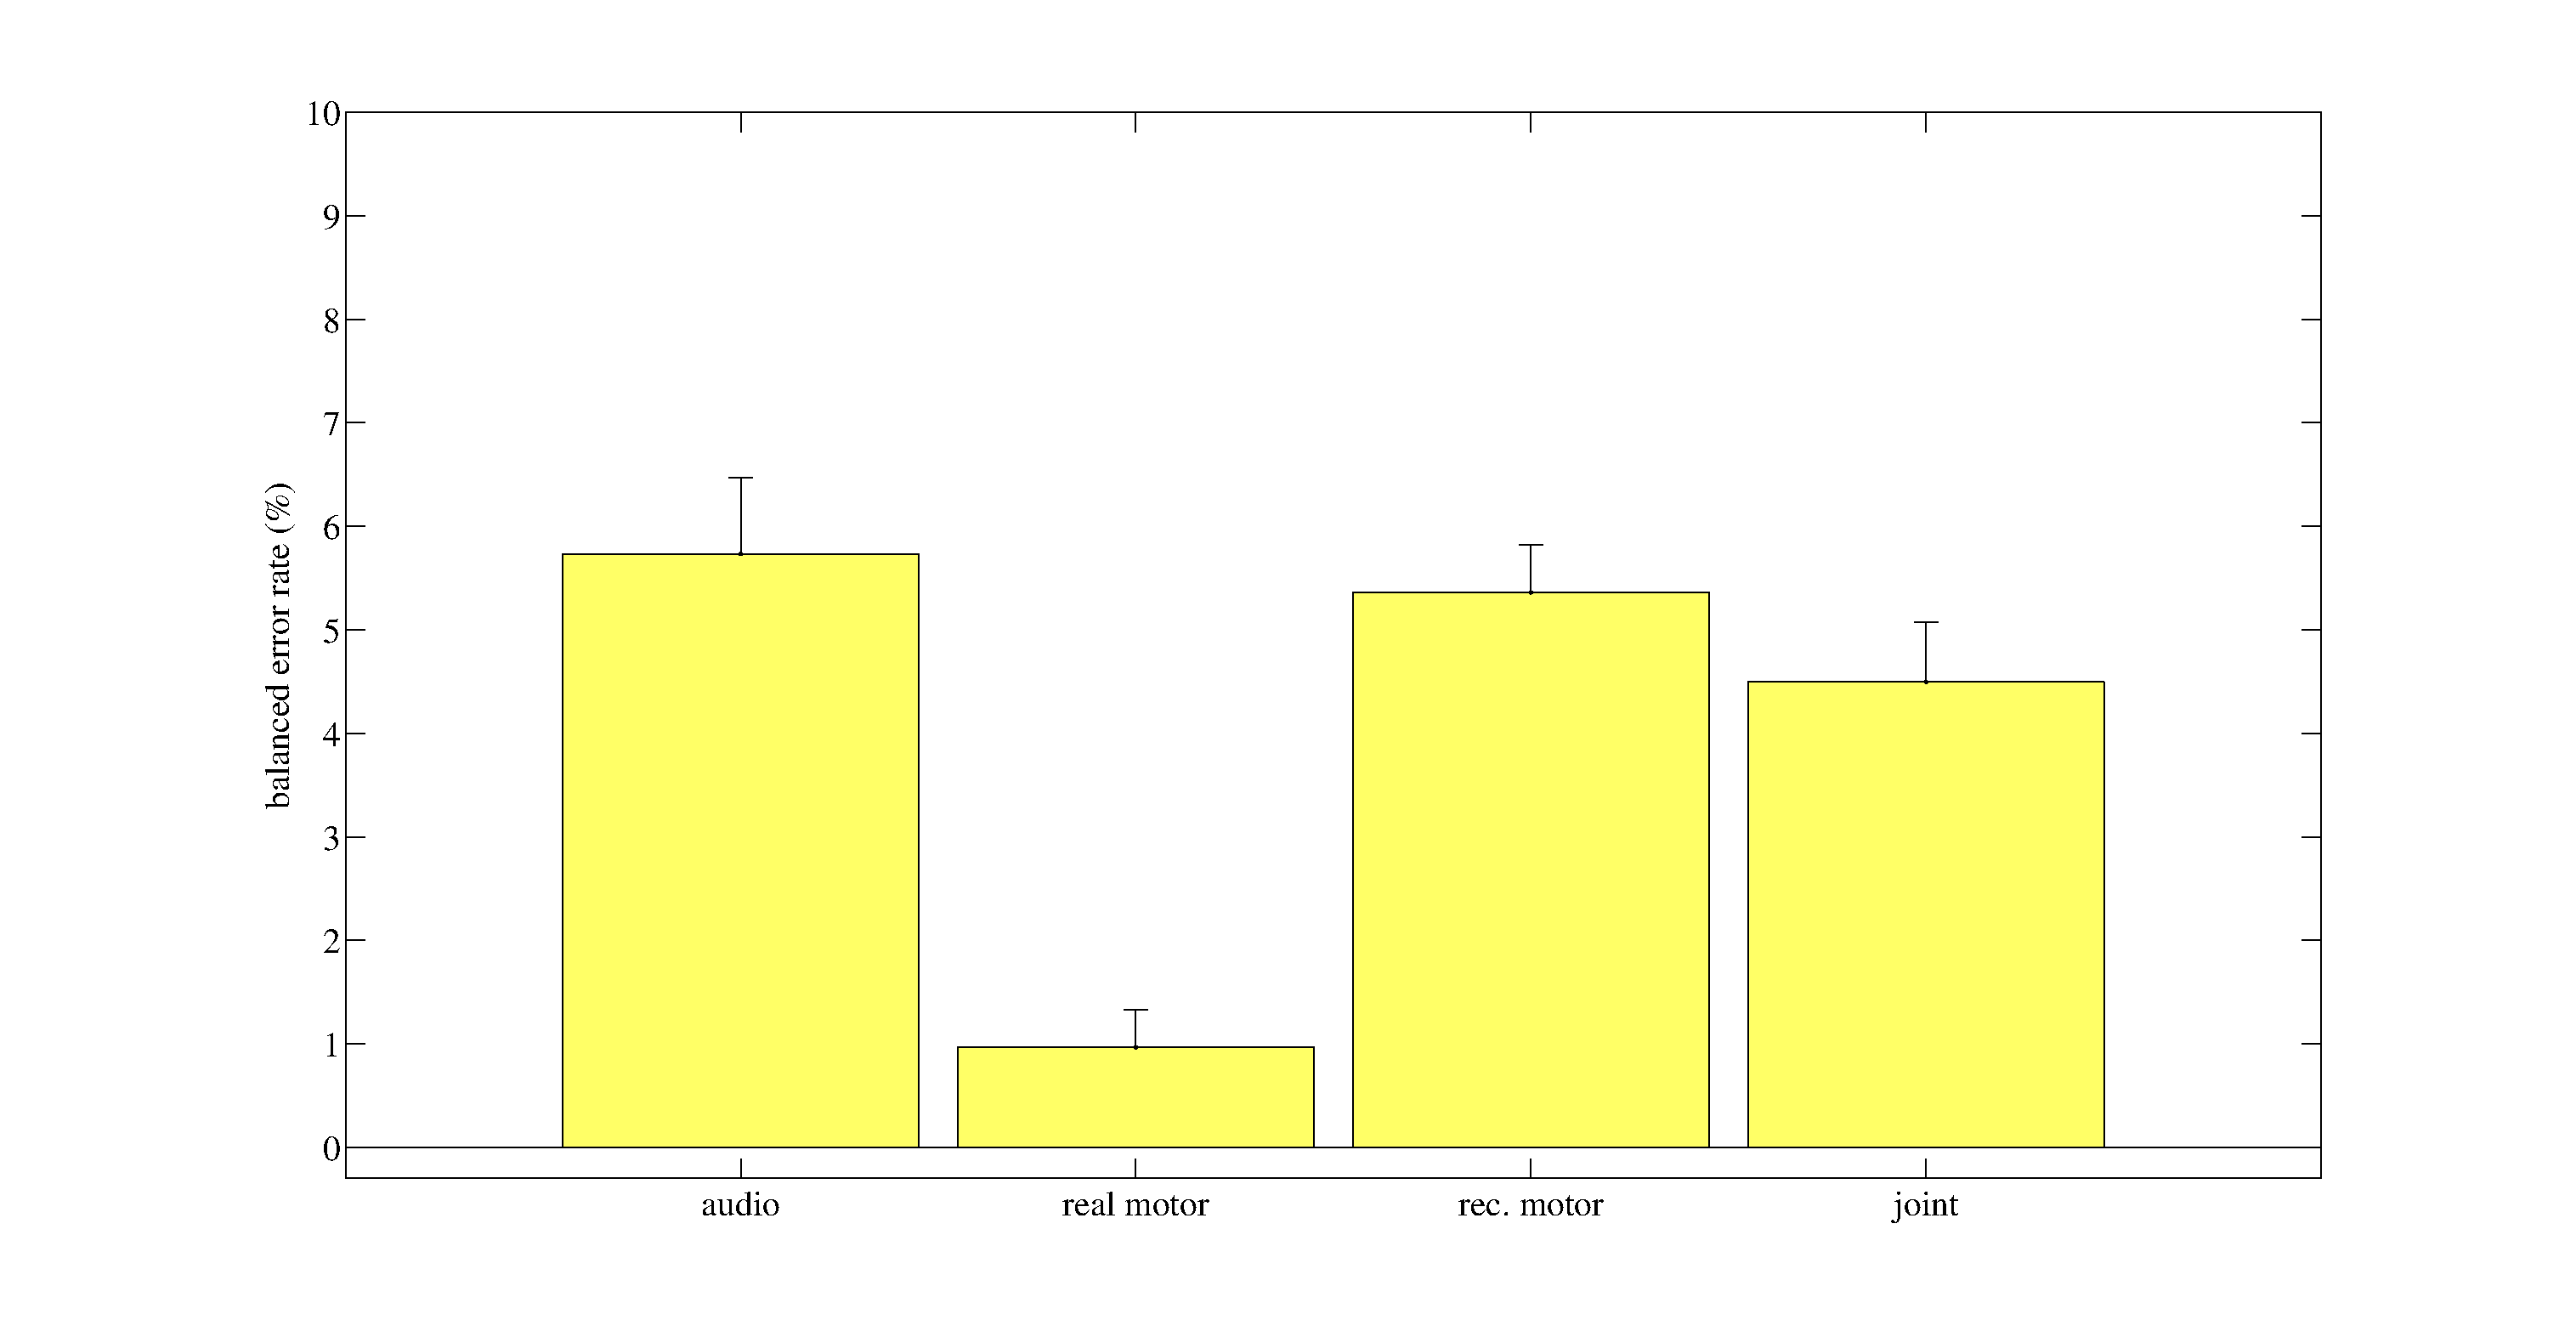
\includegraphics[width=0.95\linewidth]{figs/exp1}
  \caption{Classification results: Difference in performance between \emph{NoAdapt} and our method  on the
 classification of the grasp types.}
  \label{fig:diff_cla}
\end{figure}

\begin{figure*}[ht] \centering
  \begin{tabular}{cc}
    \includegraphics[width=0.45\textwidth]{figs/exp1_abs_best} &
    \includegraphics[width=0.45\textwidth]{figs/exp1_abs_worst} \\
    $(a)$ & $(b)$ \\
  \end{tabular}
  \caption{Classification results: $(a)$ Best classification rate gain of the adapted model compared to
 \emph{NoAdapt} and \emph{Prior} on a particular subject; $(b)$ worst performance on another subject.}
  \label{fig:cla_abs}
\end{figure*}

\begin{figure}[ht]
  \centering
  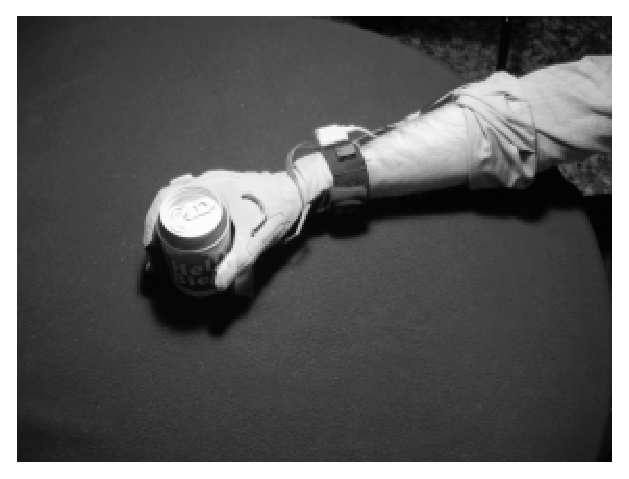
\includegraphics[width=0.95\linewidth]{figs/exp2}
  \caption{Regression experiments: Difference in performance between \emph{NoAdapt} and our method  on the
 regression of the force.}
  \label{fig:diff_reg}
\end{figure}

\begin{figure*}[ht] \centering
  \begin{tabular}{cc}
    \includegraphics[width=0.45\textwidth]{figs/exp2_abs_best} &
    \includegraphics[width=0.45\textwidth]{figs/exp2_abs_worst} \\
    $(a)$ & $(b)$ \\
  \end{tabular}
  \caption{Regression experiments: $(a)$ Best correlation coefficient gain of the adapted model compared to \emph{NoAdapt}
 and \emph{Prior} on a particular subject; $(b)$ worst performance on another subject.}
  \label{fig:reg_abs}
\end{figure*}


\subsection{Grasp Classification}
\label{subsec:classification}
\input{31.class}

\subsection{EMG to Force Regression}
\label{subsec:regression}
\input{32.regr}

\section{Conclusions}
\label{sec:conclusions}
The model adaptation method presented in this paper stems from a
problem in adaptive hand prosthetics, namely: is it possible to help a
patient to learn to use a dexterous hand prosthesis 
%in a quicker and
%better way, 
by exploiting the common features found in models trained upon other
patients?

The answer, at least as far as healthy subjects are concerned, is yes:
we have hereby presented a novel method for model adaptation in
machine learning, using Least-Squares SVMs; the idea is to build a SVM
solution which is \emph{close} to one of a set of pre-stored
models. The choice of which model to use among the pre-trained ones,
as well as the parameter $\beta$, determining the degree of closeness
to start the training from, are completely automatic, as we use an
estimation of the generalization error.

We tested our method on a database built with EMG and force data from
$10$ healthy subjects, trying to improve the training times and
asyntotic performance of one subject by pre-training on other
subjects. The outcome of the experiment is positive: our method gains
consistently both in the classification and regression tasks in the
best and average cases, and it resorts to the non-adaptive performance
in the worst.

Therefore, it is apparent that a large amount of knowledge stored in
LS-SVM models is common to all subjects, which is obviously due to the
analogies among the tasks performed by the subjects, as well as to the
anatomical similarities among the arms and the careful positioning of
the electrodes on the subjects' forearms. A further interesting point
is that, almost uniformly, models obtained by adaptation from a
pre-trained model obtain a \emph{better} performance than those
trained from scratch. This result is somehow surprising, although very
encouraging.

Lastly, let us consider the fact that, most likely, the overall
performance of the method will increase when more subjects are
available, since this would mean a larger probability of finding a
matching pre-trained model. In a clinical setting, this means that
after an experimental phase, adaptive prostheses employing this method
could actually be built. It remains, of course, to discover whether
this idea can be transferred to amputees: amputations are, obviously,
non-controlled, traumatic events (except in some cases), and therefore
stumps exhibit much more variability than healthy forearms. This is
the subject of ongoing as well as future research.


\section*{Acknowledgments}

This work is partially supported by the project NEURObotics,
FP6-IST-001917.

{\small
\bibliographystyle{IEEEtran}
\bibliography{paper}
}

%% \begin{IEEEbiography}{\includegraphics[width=1in,height=1.25in,clip,keepaspectratio]{claudio}}{Claudio Castellini}
%% biography
%% \end{IEEEbiography}

%% \begin{IEEEbiography}{\includegraphics[width=1in,height=1.25in,clip,keepaspectratio]{patrick}}{Patrick van der Smagt}
%% biography
%% \end{IEEEbiography}

%% \begin{IEEEbiography}{\includegraphics[width=1in,height=1.25in,clip,keepaspectratio]{claudio}}{Giulio Sandini}
%% biography
%% \end{IEEEbiography}

\end{document}
